\subsection{Анализирование энтропии в Mathematica}
\newcommand{\EntropyGfxScale}{0.8\textwidth}

(Эта часть впервые появилась в моем блоге 13-May-2015.
Обсуждение: \url{https://news.ycombinator.com/item?id=9545276}.)

Можно нарезать файл на блоки, подсчитать энтропию для каждого и построить график.
Я сделал это в Wolfram Mathematica для демонстрации, и вот исходный код (Mathematica 10):

\begin{lstlisting}[style=custommath]
(* loading the file *)
input=BinaryReadList["file.bin"];

(* setting block sizes *)
BlockSize=4096;BlockSizeToShow=256;

(* slice blocks by 4k *)
blocks=Partition[input,BlockSize];

(* how many blocks we've got? *)
Length[blocks]

(* calculate entropy for each block. 2 in Entropy[] (base) is set with the intention so Entropy[] 
function will produce the same results as Linux ent utility does *)
entropies=Map[N[Entropy[2,#]]&,blocks];

(* helper functions *)
fBlockToShow[input_,offset_]:=Take[input,{1+offset,1+offset+BlockSizeToShow}]
fToASCII[val_]:=FromCharacterCode[val,"PrintableASCII"]
fToHex[val_]:=IntegerString[val,16]
fPutASCIIWindow[data_]:=Framed[Grid[Partition[Map[fToASCII,data],16]]]
fPutHexWindow[data_]:=Framed[Grid[Partition[Map[fToHex,data],16],Alignment->Right]]

(* that will be the main knob here *)
{Slider[Dynamic[offset],{0,Length[input]-BlockSize,BlockSize}],Dynamic[BaseForm[offset,16]]}

(* main UI part *)
Dynamic[{ListLinePlot[entropies,GridLines->{{-1,offset/BlockSize,1}},Filling->Axis,AxesLabel->{"offset","entropy"}],
CurrentBlock=fBlockToShow[input,offset];
fPutHexWindow[CurrentBlock],
fPutASCIIWindow[CurrentBlock]}]
\end{lstlisting}

\subsubsection{База GeoIP \ac{ISP}}

\myindex{GeoIP}
Начнем с файла \href{https://www.maxmind.com/en/geoip-demo}{GeoIP}
(в котором информация об \ac{ISP} для каждого блока IP-адресов).
Бинарный файл \IT{GeoIPISP.dat} имеет какие-то таблицы (вероятно, интервалы IP-адресов) плюс какой-то набор текстовых строк
в конце файла (содержащий названия \ac{ISP}).

Когда загружаю его в Mathematica, вижу такое:

\begin{figure}[H]
\centering
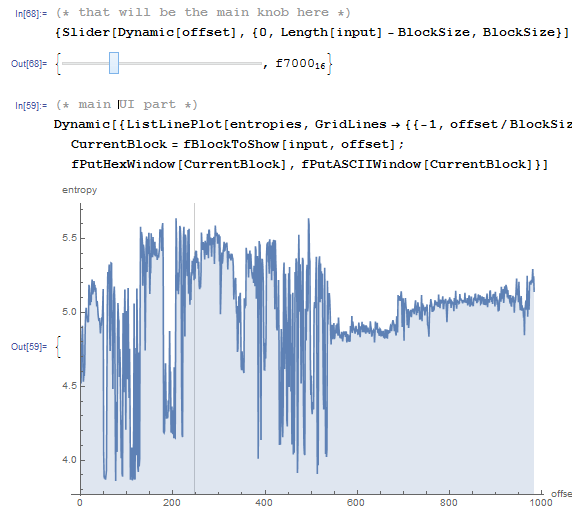
\includegraphics[width=\EntropyGfxScale]{ff/entropy/geoipisp11.png}
\end{figure}

\begin{figure}[H]
\centering
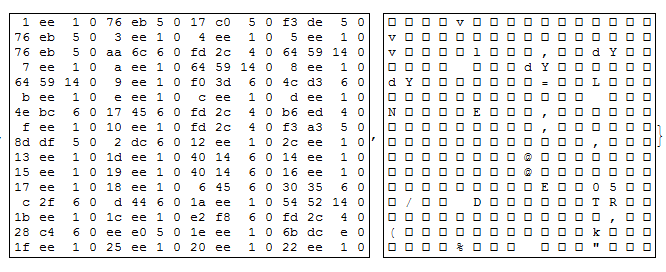
\includegraphics[width=\EntropyGfxScale]{ff/entropy/geoipisp12.png}
\end{figure}


В графике две части: первая, в каком-то смысле, хаотичная, вторая более ровная.

0 в горизонтальной оси графика означает самый низкий уровень энтропии
(данные, которые можно сжать очень сильно, \IT{упорядоченные} другими словами) 
и 8 это самый высокий (нельзя сжать вообще, \IT{хаотичные} или \IT{случайные} другими словами).
Почему 0 и 8? 0 означает 0 бит на байт (байт как контейнер не заполнен вообще) 
и 8 означает 8 бит на байт, т.е., весь байт (как контейнер) плотно заполнен информацией.

Когда я двигаю слайдер в место в середине первого блока, то ясно вижу некоторый массив из 32-битных целочисленных значений.
Потом я сдвигаю слайдер в середину второго блока и вижу текст на английском:

\begin{figure}[H]
\centering
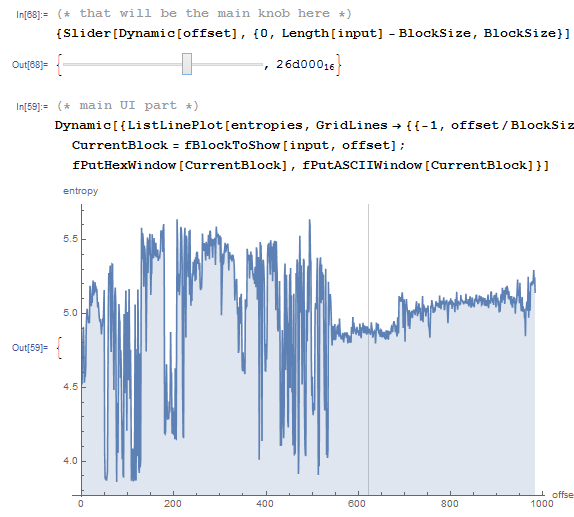
\includegraphics[width=\EntropyGfxScale]{ff/entropy/geoipisp21.png}
\end{figure}

\begin{figure}[H]
\centering
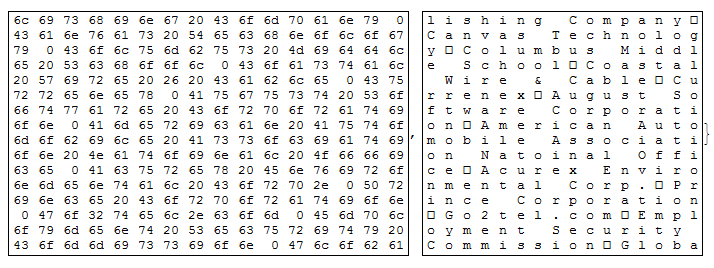
\includegraphics[width=\EntropyGfxScale]{ff/entropy/geoipisp22.png}
\end{figure}


Действительно, это названия ISP.
Так что, энтропия английского текста это 4.5-5.5 бита на байт? Да, что-то в этом роде.
В Wolfram Mathematica есть встроенный корпус хорошо известной английской литературы, и мы можем посмотреть энтропию
шейкспировских соннетов:

\begin{lstlisting}[style=custommath]
In[]:= Entropy[2,ExampleData[{"Text","ShakespearesSonnets"}]]//N
Out[]= 4.42366
\end{lstlisting}

4.4 это близко к тому, что мы получили (4.7-5.3). 
Конечно, классическая английская литература немного отличается от названий ISP и других английских текстов, которые мы
можем найти в бинарных файлах (отладочные сообщения, сообщения об ошибках), но это значение близко.

\subsubsection{Прошивка TP-Link WR941}

Следующий пример. Вот прошивка от роутера TP-Link WR941:

\begin{figure}[H]
\centering
\includegraphics[width=\EntropyGfxScale]{ff/entropy/tplink.png}
\end{figure}


Мы тут видим 3 блока с пустыми лакунами.
Затем, первый блок с большой энтропией (начиная с адреса 0) маленький,
второй (с адресом где-то на 0x22000) больше и третий (адрес 0x123000) самый
большой.
Не уверен насчет точного уровня энтропии первого блока, но второй и третий имеют большой уровень, означая что эти блоки
или сжаты и/или зашифрованы.

\myindex{Binwalk}
Я попробовал \href{http://binwalk.org/}{binwalk} для этого файла с прошивкой:

\begin{lstlisting}
DECIMAL       HEXADECIMAL     DESCRIPTION
--------------------------------------------------------------------------------
0             0x0             TP-Link firmware header, firmware version: 0.-15221.3, image version: "", product ID: 0x0, product version: 155254789, kernel load address: 0x0, kernel entry point: 0x-7FFFE000, kernel offset: 4063744, kernel length: 512, rootfs offset: 837431, rootfs length: 1048576, bootloader offset: 2883584, bootloader length: 0
14832         0x39F0          U-Boot version string, "U-Boot 1.1.4 (Jun 27 2014 - 14:56:49)"
14880         0x3A20          CRC32 polynomial table, big endian
16176         0x3F30          uImage header, header size: 64 bytes, header CRC: 0x3AC66E95, created: 2014-06-27 06:56:50, image size: 34587 bytes, Data Address: 0x80010000, Entry Point: 0x80010000, data CRC: 0xDF2DBA0B, OS: Linux, CPU: MIPS, image type: Firmware Image, compression type: lzma, image name: "u-boot image"
16240         0x3F70          LZMA compressed data, properties: 0x5D, dictionary size: 33554432 bytes, uncompressed size: 90000 bytes
131584        0x20200         TP-Link firmware header, firmware version: 0.0.3, image version: "", product ID: 0x0, product version: 155254789, kernel load address: 0x0, kernel entry point: 0x-7FFFE000, kernel offset: 3932160, kernel length: 512, rootfs offset: 837431, rootfs length: 1048576, bootloader offset: 2883584, bootloader length: 0
132096        0x20400         LZMA compressed data, properties: 0x5D, dictionary size: 33554432 bytes, uncompressed size: 2388212 bytes
1180160       0x120200        Squashfs filesystem, little endian, version 4.0, compression:lzma, size: 2548511 bytes, 536 inodes, blocksize: 131072 bytes, created: 2014-06-27 07:06:52
\end{lstlisting}

\myindex{LZMA}
Действительно: в начале есть что-то, но два больших блока сжатых LZMA начинаются на 0x20400 и 0x120200.
Это примерно те же адреса, что мы видим в Mathematica.
И кстати, binwalk тоже может показывать информацию об энтропии (опция \TT{-E}):

\begin{lstlisting}
DECIMAL       HEXADECIMAL     ENTROPY
--------------------------------------------------------------------------------
0             0x0             Falling entropy edge (0.419187)
16384         0x4000          Rising entropy edge (0.988639)
51200         0xC800          Falling entropy edge (0.000000)
133120        0x20800         Rising entropy edge (0.987596)
968704        0xEC800         Falling entropy edge (0.508720)
1181696       0x120800        Rising entropy edge (0.989615)
3727360       0x38E000        Falling entropy edge (0.732390)
\end{lstlisting}

Передние фронты соответствуют передним фронтам блока на нашем графе.
Задние фронты соответствуют местам, где начинаются пустые лакуны.

Binwalk также может генерировать графики в PNG (\TT{-E -J}):

\begin{figure}[H]
\centering
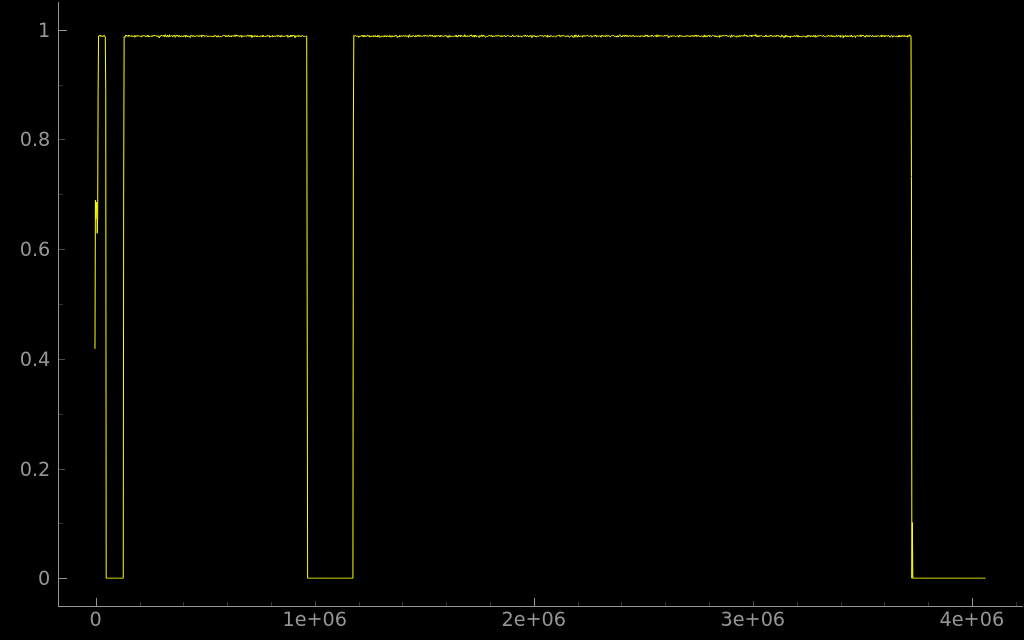
\includegraphics[width=\EntropyGfxScale]{ff/entropy/tplink_binwalk.png}
\end{figure}


Что можно сказать о лакунах? Глядя в бинарном редакторе, мы видим что они просто заполнены байтами 0xFF.
Зачем разработчики оставили эти места?
Вероятно, потому что они не могли расчитать точные размеры сжатых блоков, так что они выделили место с запасом.

\subsubsection{Notepad}

\myindex{Notepad}

Еще один пример это notepad.exe, который я взял из Windows 8.1:

\begin{figure}[H]
\centering
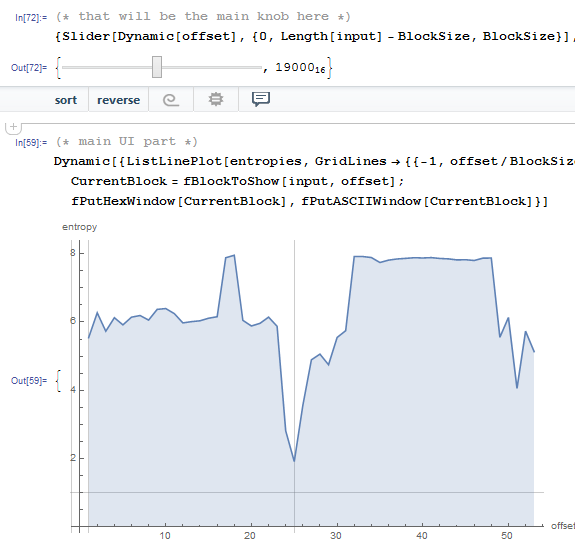
\includegraphics[width=\EntropyGfxScale]{ff/entropy/notepad11.png}
\end{figure}

\begin{figure}[H]
\centering
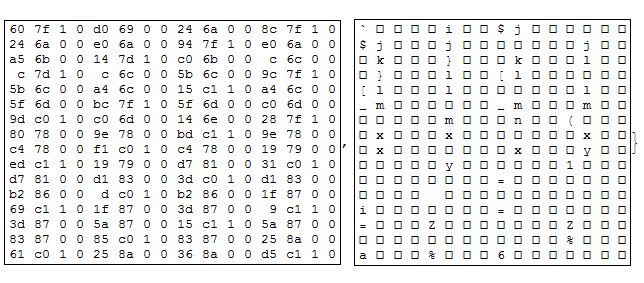
\includegraphics[width=\EntropyGfxScale]{ff/entropy/notepad12.png}
\end{figure}


Имеется углубление на $\approx 0x19000$ (абсолютное смещение в файле).
Я открыл этот исполняемый файл в шестнадцатеричном редакторе и нашел там таблицу импортов (которая имеет уровень энтропии
ниже, чем код x86-64 code в первой половине графика).

Имеется также блок с высоким уровнем энтропии, начинающийся на $\approx 0x20000$:

\begin{figure}[H]
\centering
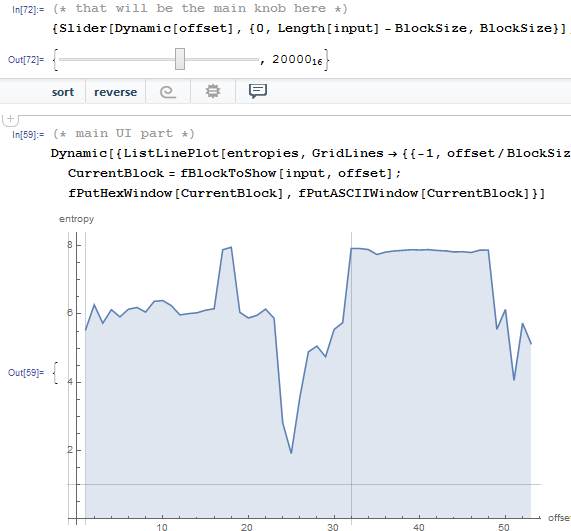
\includegraphics[width=\EntropyGfxScale]{ff/entropy/notepad21.png}
\end{figure}

\begin{figure}[H]
\centering
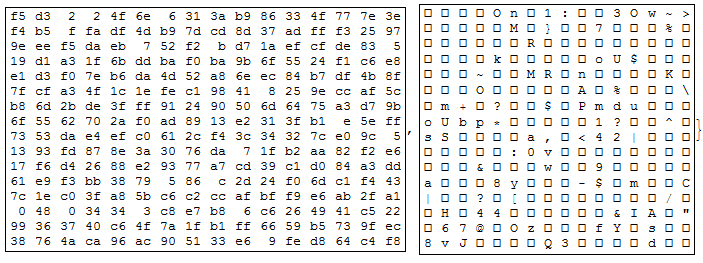
\includegraphics[width=\EntropyGfxScale]{ff/entropy/notepad22.png}
\end{figure}


\myindex{PNG}
В шестнадцатеричном редакторе можно найти там PNG-файл, вставленный в секцию ресурсов PE-файла (это большое изображение
иконки notepad-а).
Действительно, PNG-файлы ведь сжаты.

\subsubsection{Безымянный видеорегистратор}

Теперь самый продвинутый пример в этой части это прошивка от какого-то безымянного видеорегистратора,
которую мне прислал друг:

\begin{figure}[H]
\centering
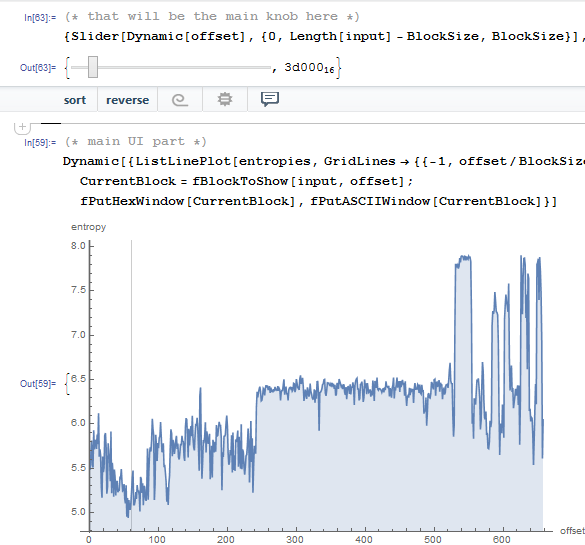
\includegraphics[width=\EntropyGfxScale]{ff/entropy/dashcam_text1.png}
\end{figure}

\begin{figure}[H]
\centering
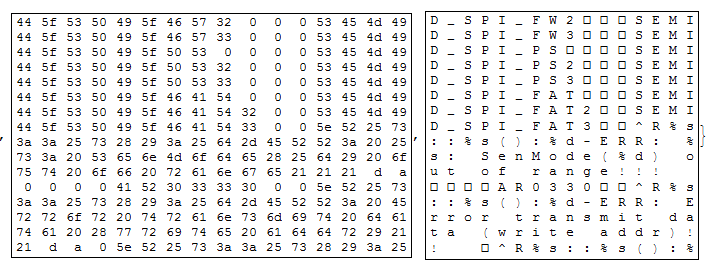
\includegraphics[width=\EntropyGfxScale]{ff/entropy/dashcam_text2.png}
\end{figure}


Спад в самом начале это текст на английском: отладочные сообщения.
\myindex{MIPS}
Я попробовал разные \ac{ISA} и нашел, что первая треть всего файла (с сегментом текста внутри) это на самом деле
код для MIPS (little-endian).

Например, это очень заметный эпилог ф-ции в MIPS-коде:

\begin{lstlisting}[style=customasmMIPS]
ROM:000013B0                 move    $sp, $fp
ROM:000013B4                 lw      $ra, 0x1C($sp)
ROM:000013B8                 lw      $fp, 0x18($sp)
ROM:000013BC                 lw      $s1, 0x14($sp)
ROM:000013C0                 lw      $s0, 0x10($sp)
ROM:000013C4                 jr      $ra
ROM:000013C8                 addiu   $sp, 0x20
\end{lstlisting}

Из нашего графика мы видим, что энтропия кода для MIPS 5-6 бит на байт.
Действительно, я измерил энтропию кода для различных \ac{ISA} и получил такие значения:

\begin{itemize}
\item x86: секция .text в файле ntoskrnl.exe из Windows 2003: 6.6
\item x64: секция .text в файле ntoskrnl.exe из Windows 7 x64: 6.5
\item ARM (режим thumb), Angry Birds Classic: 7.05
\item ARM (режим ARM) Linux Kernel 3.8.0: 6.03
\item MIPS (little endian), секция .text файла user32.dll из Windows NT 4: 6.09
\end{itemize}

Энтропия исполняемого кода выше чем у текста на английском, но всё равно можно сжимать.

Теперь вторая треть, начинающаяся с 0xF5000. Я не знаю, что это. Пробовал различные \ac{ISA} без всякого успеха.
Энтропия этого блока выглядит ровнее, чем у блока с исполняемым кодом.
Может это какие-то данные?

\myindex{JPEG}
Имеется также всплеск на $\approx 0x213000$.
Я посмотрел на это место в бинарном редакторе и нашел JPEG-файл (который, конечно же, сжат)!
Также, я не знаю, что находится в конце.
Попробуем Binwalk на этом файле:

\begin{lstlisting}
% binwalk FW96650A.bin 

DECIMAL       HEXADECIMAL     DESCRIPTION
--------------------------------------------------------------------------------
167698        0x28F12         Unix path: /15/20/24/25/30/60/120/240fps can be served..
280286        0x446DE         Copyright string: "Copyright (c) 2012 Novatek Microelectronic Corp."
2169199       0x21196F        JPEG image data, JFIF standard 1.01
2300847       0x231BAF        MySQL MISAM compressed data file Version 3

% binwalk -E FW96650A.bin 

DECIMAL       HEXADECIMAL     ENTROPY
--------------------------------------------------------------------------------
0             0x0             Falling entropy edge (0.579792)
2170880       0x212000        Rising entropy edge (0.967373)
2267136       0x229800        Falling entropy edge (0.802974)
2426880       0x250800        Falling entropy edge (0.846639)
2490368       0x260000        Falling entropy edge (0.849804)
2560000       0x271000        Rising entropy edge (0.974340)
2574336       0x274800        Rising entropy edge (0.970958)
2588672       0x278000        Falling entropy edge (0.763507)
2592768       0x279000        Rising entropy edge (0.951883)
2596864       0x27A000        Falling entropy edge (0.712814)
2600960       0x27B000        Rising entropy edge (0.968167)
2607104       0x27C800        Rising entropy edge (0.958582)
2609152       0x27D000        Falling entropy edge (0.760989)
2654208       0x288000        Rising entropy edge (0.954127)
2670592       0x28C000        Rising entropy edge (0.967883)
2676736       0x28D800        Rising entropy edge (0.975779)
2684928       0x28F800        Falling entropy edge (0.744369)
\end{lstlisting}

Да, она нашла JPEG-файл и даже данные для MySQL!
Но я не уверен что это правда --- пока не проверял.

\myindex{кластеризация}
Также интересно попробовать кластеризацию в Mathematica:

\begin{figure}[H]
\centering
\includegraphics[width=\EntropyGfxScale]{ff/entropy/dashcam_clusters.png}
\end{figure}


Это пример, как Mathematica группирует различные значения энтропии в различимые группы.
Действительно, похоже на правду. Синие точки в районе 5.0-5.5, вероятно относятся к тексту на английском.
Желтые точки в 5.5-6 это код для MIPS. Множество зеленых точек в 6.0-6.5 это неизвестная вторая треть.
Оранжевые точки близкие к 8.0 относятся к сжатому JPEG-файлу.
Другие оранжевые точки, видимо, относятся к концу прошивки (неизвестные для нас данные).

\subsubsection{Ссылки}

Бинарные файлы, которые использовались в этой части:
\url{https://github.com/dennis714/RE-for-beginners/tree/master/ff/entropy/files}.
Файл для Wolfram Mathematica: \url{https://github.com/dennis714/RE-for-beginners/blob/master/ff/entropy/files/binary_file_entropy.nb}
(все ячейки должны быть в начале проинициализированы, что всё начало работать).

